\section{.NET Grundlagen}

\subsection{Memory Layout}
Klassen werden auf dem Heap angelegt und sind implizit public. Structs werden auf dem Stack angelegt und sind implizit public. \\
\begin{minipage}{0,33\linewidth}
\begin{lstlisting}
// Example 1
public struct Student
{
	public Exam exam;
}
public class Exam
{
	public int grade;
}
\end{lstlisting}  
\end{minipage}
\begin{minipage}{0,33\linewidth}
\begin{lstlisting}
// Example 2
public class Student
{
	public Exam Math;
}
public struct Exam
{
	public int Grade;
}
\end{lstlisting}  
\end{minipage}
\begin{minipage}{0,33\linewidth}
\begin{lstlisting}
public static void Test()
{
	Exam ex1 = new Exam();
	ex1.grade = 3;
	
	Student s1 = new Student();
	Student s2 = s1;
	s1.exam = ex1;
	ex1.grade = 5;
}
\end{lstlisting}
\end{minipage}

\begin{minipage}{0,5\linewidth}
	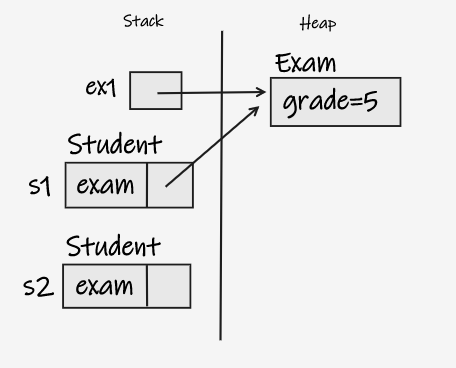
\includegraphics[width=0.75\linewidth]{ml1}
\end{minipage}
\begin{minipage}{0,5\linewidth}
 	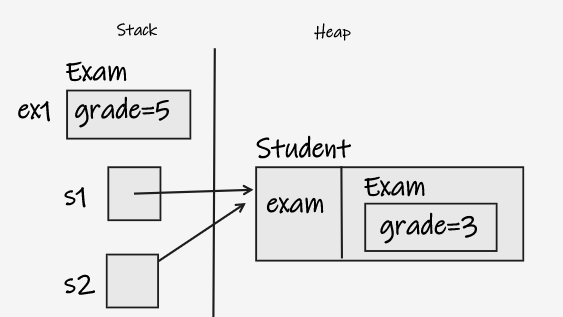
\includegraphics[width=0.75\linewidth]{ml2}
\end{minipage}
